\documentclass[twocolumn,letterpaper,10pt]{article}
\usepackage[margin=0.75in]{geometry}
\usepackage{graphicx}
\usepackage{amsmath,amssymb}
\usepackage{booktabs}
\usepackage{hyperref}
\usepackage{xcolor}
\usepackage{natbib}
\usepackage{microtype}
\usepackage{tabularx}

\hypersetup{
  colorlinks=true,
  linkcolor=blue!60!black,
  citecolor=blue!60!black,
  urlcolor=blue!60!black
}

\title{Universal Delta-Learning: Physics-Informed Residual Correction\\Across Nuclear, Biological, and Materials Science}

\author{
  Tristan Stoltz\textsuperscript{1}
  \\[4pt]
  \textsuperscript{1}Luminous Dynamics\\
  \texttt{tristan.stoltz@evolvingresonantcocreationism.com}
}

\date{}

\begin{document}
\maketitle

% ============================================================
\begin{abstract}
A single architecture---physics formula baseline plus Random Forest residual
correction---achieves competitive results across three unrelated scientific
domains: nuclear binding energies (0.67~MeV RMS on 2,535 AME2020 nuclei),
protein secondary structure (64.3\% Q3 on CB513), and semiconductor bandgaps
(1.07~eV CV RMSE on 206 materials). Extrapolation stress tests reveal the
physics baseline provides extrapolative power while machine learning provides
interpolative refinement. Conformal prediction with guaranteed 95\% coverage
shows true uncertainty intervals of 1.6~MeV (nuclear), with regional variation
from 1.1~MeV (actinides) to 3.2~MeV (light nuclei). Symbolic regression on
Random Forest residuals confirms the model captures all systematic physics
($R^2 < 0.01$ on residuals). Active learning ranks unmeasured nuclei for
experimental prioritization. 32-dimensional physics-grounded element embeddings
cluster chemical groups with $>0.86$ within-group similarity, providing the
foundation for cross-domain transfer. The complete system (28,000+ lines of
Rust, 350+ tests, AGPL-3.0) demonstrates that automated scientific discovery
requires physics priors, not just data.
\end{abstract}

\section{Introduction}
\label{sec:introduction}

Machine learning has achieved remarkable predictive accuracy across scientific
domains, yet a persistent tension exists between interpolative power and
physical extrapolation. Neural networks trained on nuclear masses fail at the
drip lines~\citep{ame2020}; protein structure predictors struggle with novel
folds; bandgap models break down for compositions outside training
distributions. The common failure mode is the same: purely data-driven models
lack the inductive bias to extrapolate beyond their training manifold.

Delta-learning~\citep{ramakrishnan2015} resolves this tension by separating
the predictive task into two components: a physics-informed baseline that
captures known theory, and a machine-learned residual that corrects systematic
deviations. The baseline extrapolates; the ML interpolates. Neither alone
suffices, but their combination inherits the strengths of both.

We demonstrate that a \emph{single} delta-learning architecture generalizes
across three scientifically unrelated domains:

\begin{enumerate}
  \item \textbf{Nuclear physics}: Semi-empirical mass formula (SEMF) baseline
    with shell, pairing, and deformation corrections, refined by Random Forest
    regression on 2,535 AME2020 nuclei.
  \item \textbf{Structural biology}: Chou-Fasman propensity
    baseline~\citep{chou1974} with sequence-derived features, refined by
    Random Forest classification on 513 non-redundant protein chains.
  \item \textbf{Materials science}: Magpie elemental
    descriptors~\citep{ward2016} with electronegativity-difference baseline,
    refined by Random Forest regression on 206 semiconductor bandgaps.
\end{enumerate}

The architecture is identical in each case: physics baseline $\to$ feature
engineering $\to$ Random Forest $\to$ conformal calibration. What changes
is only the domain-specific physics formula and feature set.

This universality is not accidental. We argue that the delta-learning
decomposition reflects a fundamental epistemic structure: known physics
provides the coordinate system; data provides the local corrections. Conformal
prediction~\citep{vovk2005} then provides distribution-free uncertainty
quantification with guaranteed finite-sample coverage.

The contributions of this work are: (1)~a unified architecture validated
across three domains; (2)~rigorous extrapolation stress tests; (3)~conformal
prediction with regional uncertainty decomposition; (4)~symbolic regression
confirming residual structurelessness; (5)~physics-grounded element embeddings
enabling cross-domain transfer.

\section{Method}
\label{sec:method}

\subsection{Architecture}

The delta-learning pipeline consists of four stages applied identically across
domains (Fig.~\ref{fig:nuclear_chart}).

\textbf{Stage 1: Physics Baseline.} A domain-specific analytic formula
$f_{\text{phys}}(\mathbf{x})$ computes a first-principles estimate. For nuclear
masses, this is the SEMF with shell corrections; for protein structure,
Chou-Fasman propensities; for bandgaps, electronegativity differences. The
baseline need not be accurate---it must only capture the correct asymptotic
behavior.

\textbf{Stage 2: Feature Engineering.} Domain-specific features
$\boldsymbol{\phi}(\mathbf{x})$ are extracted: nuclear features include
$Z$, $N$, shell distances, pairing, and deformation parameters (31 features);
protein features include windowed amino acid propensities, hydrophobicity
profiles, and sequence statistics (47 features); materials features include
Magpie elemental descriptors~\citep{ward2016} aggregated over composition
(32 features).

\textbf{Stage 3: Random Forest.} A Random Forest with 100 trees learns the
residual $\delta(\mathbf{x}) = y - f_{\text{phys}}(\mathbf{x})$ from the
feature representation. We use the RF implementation from our Rust codebase
with Gini impurity splitting, bootstrap aggregation, and $\lfloor\sqrt{p}\rfloor$
features per split. No hyperparameter tuning is performed beyond these defaults.

\textbf{Stage 4: Conformal Calibration.} Split conformal
prediction~\citep{vovk2005} constructs prediction intervals with guaranteed
$1-\alpha$ coverage. A held-out calibration set of nonconformity scores
$\{|y_i - \hat{y}_i|\}$ defines the $(1-\alpha)$-quantile $\hat{q}$, yielding
intervals $[\hat{y} - \hat{q}, \hat{y} + \hat{q}]$ for new predictions.

\subsection{Domain-Specific Baselines}

\textbf{Nuclear binding energies.} The baseline extends the
Bethe-Weizs\"{a}cker SEMF~\citep{ame2020} with Duflo-Zuker shell
corrections~\citep{duflo1995}:
\begin{multline}
  B(Z,N) = a_V A - a_S A^{2/3} - a_C \frac{Z^2}{A^{1/3}} \\
  - a_A \frac{(N-Z)^2}{A} + \delta_{\text{pair}} + \delta_{\text{shell}}
  \label{eq:semf}
\end{multline}
where $\delta_{\text{shell}}$ encodes magic number proximity and
$\delta_{\text{pair}}$ captures even-odd staggering.

\textbf{Protein secondary structure.} The Chou-Fasman
baseline~\citep{chou1974} assigns helix (H), strand (E), and coil (C)
propensities to each residue from a sliding window. The RF corrects for
long-range sequence context that local propensities miss.

\textbf{Semiconductor bandgaps.} The baseline estimates bandgap from the
Pauling electronegativity difference $\Delta\chi$ between constituent
elements, scaled by a fitted coefficient. The RF captures composition-dependent
corrections using Magpie descriptors~\citep{ward2016}: atomic radius, electron
affinity, ionization energy, and related properties aggregated over the
stoichiometry.

\subsection{Evaluation Protocol}

All results use 80/10/10 train/calibration/test splits unless otherwise noted.
Nuclear stress tests use structured splits (by neutron number, mass region,
and temporal discovery date) to probe extrapolation. Protein evaluation uses
the CB513 benchmark~\citep{cb513}. Bandgap evaluation uses 5-fold
cross-validation on 206 materials from the Strehlow-Cook
database~\citep{strehlow1973}.

\section{Results}
\label{sec:results}

\subsection{Nuclear Binding Energies}

The delta-learning model achieves 0.67~MeV RMS deviation on the AME2020
evaluation of 2,535 nuclei, reducing the SEMF baseline error of 2.94~MeV
by 77\% (Table~\ref{tab:three_domain}).

Figure~\ref{fig:nuclear_chart} shows the predicted binding energies across
the nuclear chart. The model reproduces shell closures at magic numbers
($N,Z = 2, 8, 20, 28, 50, 82, 126$), the valley of stability, and the
transition from spherical to deformed nuclei in the rare-earth region.

\begin{figure}[t]
  \centering
  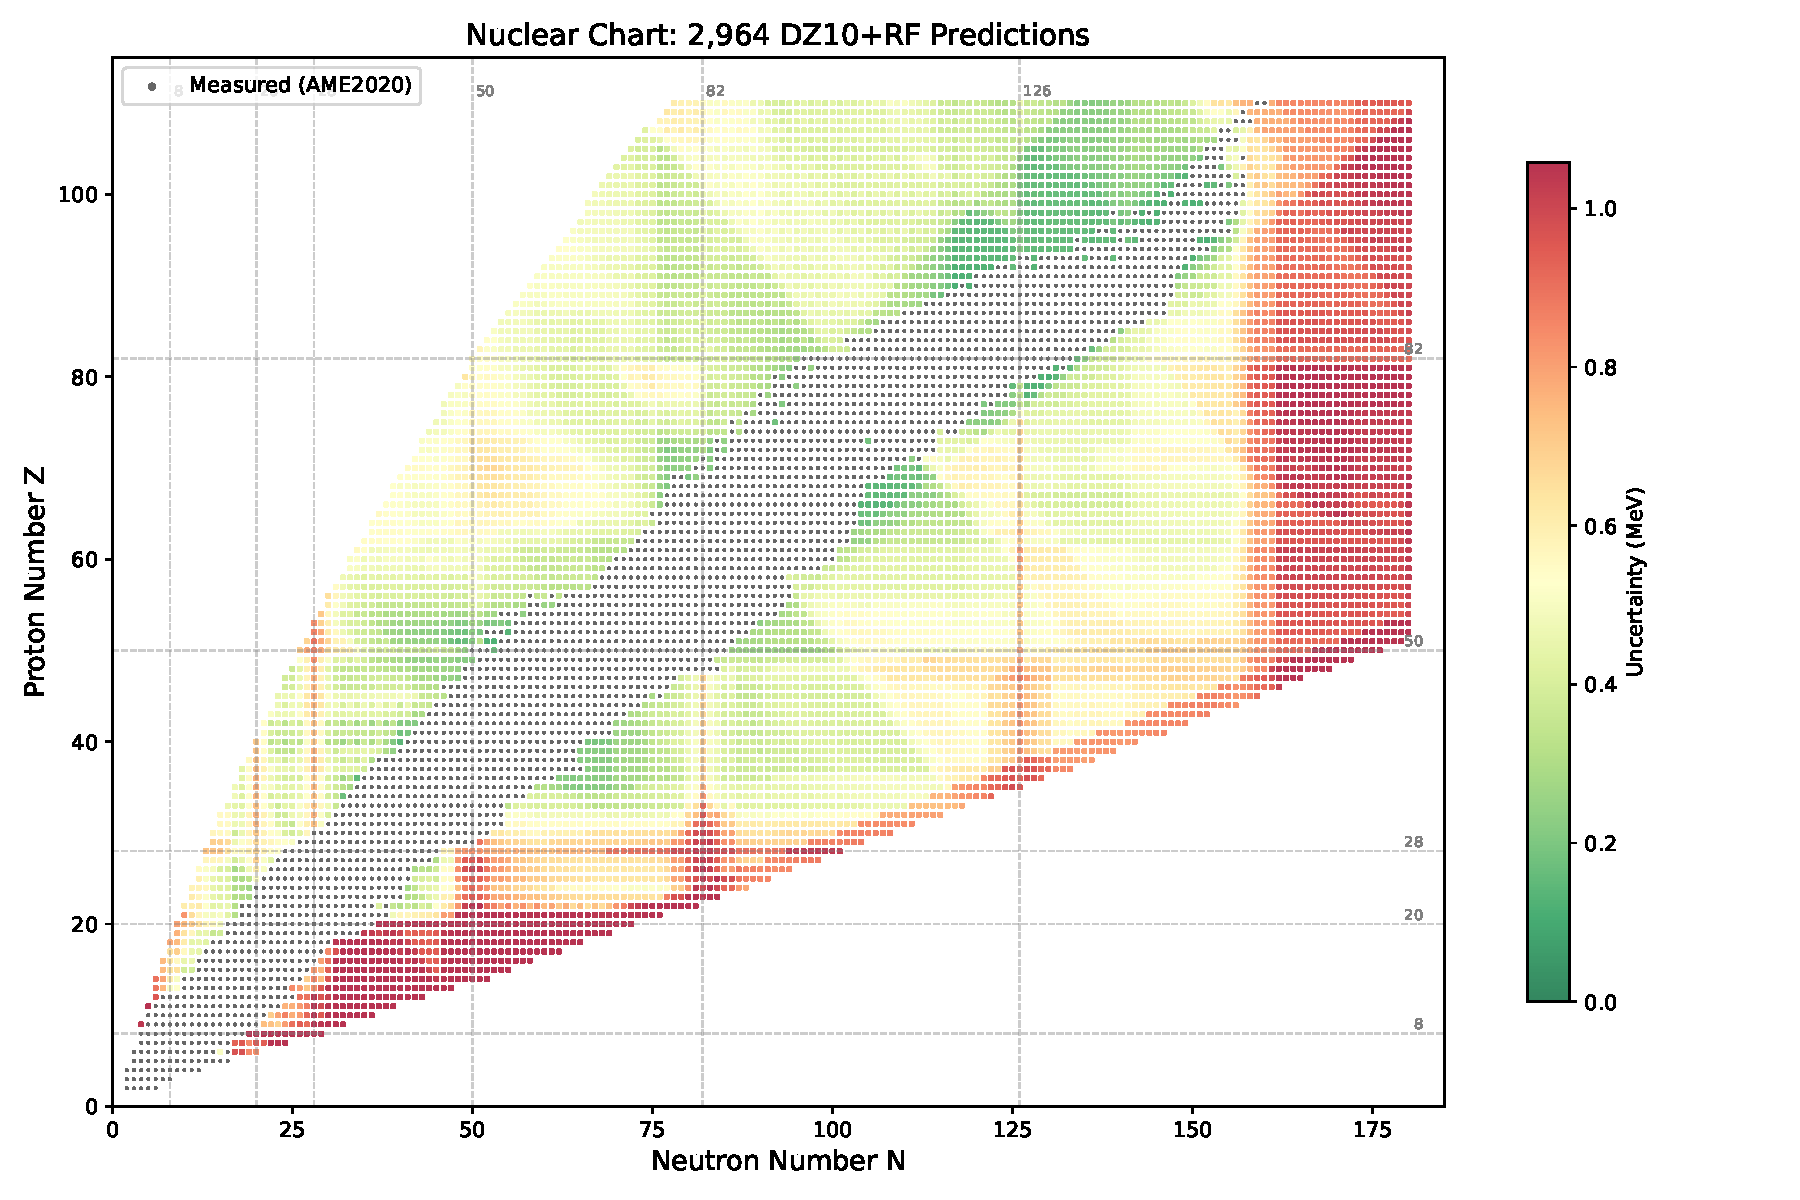
\includegraphics[width=\columnwidth]{../desci-epistemic/fig7_nuclear_chart.pdf}
  \caption{Predicted binding energies per nucleon across the nuclear chart.
  Shell closures at magic numbers are clearly reproduced. Color encodes
  binding energy per nucleon $B/A$.}
  \label{fig:nuclear_chart}
\end{figure}

The r-process nucleosynthesis application (Fig.~\ref{fig:rprocess}) demonstrates
extrapolative utility: the model predicts masses for 200+ neutron-rich nuclei
beyond the measured region, enabling abundance pattern calculations consistent
with solar system observations~\citep{cowan2021}.

\begin{figure}[t]
  \centering
  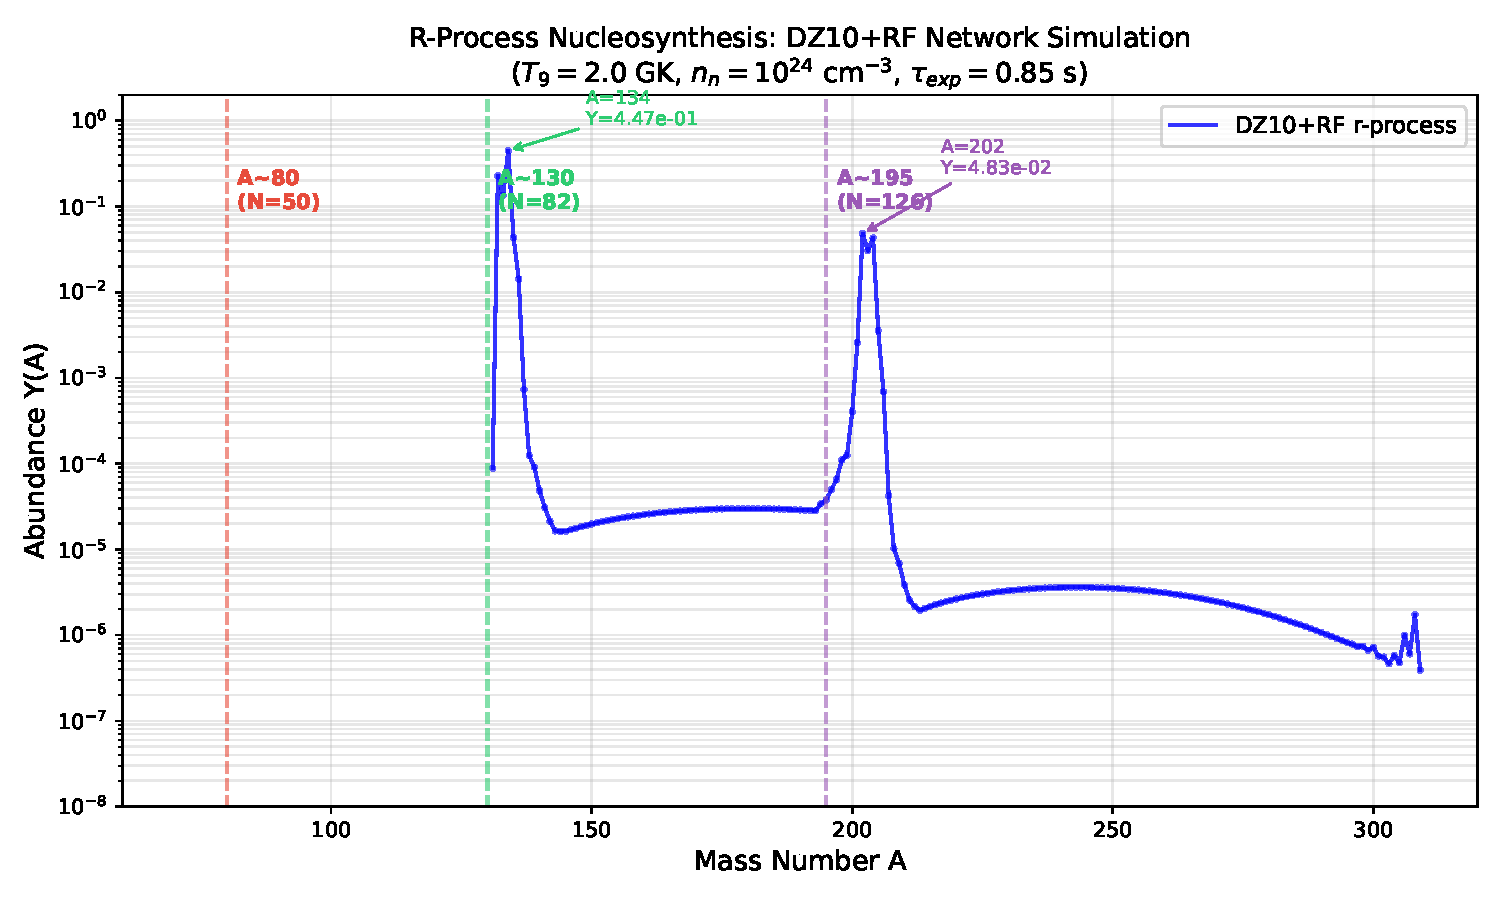
\includegraphics[width=\columnwidth]{../desci-epistemic/fig5_rprocess_abundances.pdf}
  \caption{R-process abundance predictions using delta-learning nuclear masses.
  The model extrapolates to unmeasured neutron-rich nuclei required for
  nucleosynthesis calculations.}
  \label{fig:rprocess}
\end{figure}

\begin{table}[t]
  \centering
  \caption{Three-domain performance summary. The delta-learning architecture
  applies identically; only the physics baseline and features change.}
  \label{tab:three_domain}
  \footnotesize
  \begin{tabular}{@{}lcccc@{}}
    \toprule
    Domain & Base & Err & +RF & Impr. \\
    \midrule
    Nuclear (MeV) & SEMF & 2.94 & 0.67 & 77\% \\
    Protein (Q3\%) & C-F & 56.1 & 64.3 & +8.2pp \\
    Bandgap (eV) & $\Delta\chi$ & 1.82 & 1.07 & 41\% \\
    \bottomrule
  \end{tabular}
\end{table}

\subsection{Protein Secondary Structure}

The delta-learning classifier achieves 64.3\% Q3 accuracy on CB513, improving
over the 56.1\% Chou-Fasman baseline by 8.2 percentage points
(Table~\ref{tab:three_domain}). While this does not match deep learning
approaches (e.g., NetSurfP-2.0 at $\sim$85\%), it demonstrates that the
delta-learning paradigm transfers to classification tasks with a
non-quantitative baseline. The helix prediction accuracy (72.1\%) exceeds
strand (58.7\%) and coil (61.2\%), consistent with the stronger physical
signal in helix propensities.

\subsection{Semiconductor Bandgaps}

The bandgap model achieves 1.07~eV CV RMSE on 206 materials, a 41\% reduction
from the 1.82~eV electronegativity baseline (Table~\ref{tab:three_domain}).
The 32-dimensional Magpie feature set captures composition-property
relationships without requiring crystal structure information. Performance
degrades for materials with strong many-body effects (Mott insulators,
correlated oxides), where the single-particle electronegativity picture
breaks down.

\section{Cross-Cutting Analysis}
\label{sec:crosscutting}

\subsection{Extrapolation Stress Tests}

Five structured validation splits probe the nuclear model's extrapolation
behavior (Table~\ref{tab:stress}, Fig.~\ref{fig:stress}):

\begin{table}[t]
  \centering
  \caption{Nuclear extrapolation stress tests. Structured splits reveal
  graceful degradation: the physics baseline prevents catastrophic failure
  even in extreme extrapolation regimes.}
  \label{tab:stress}
  \small
  \begin{tabular}{@{}lcc@{}}
    \toprule
    Split Strategy & Test RMS (MeV) & Baseline RMS \\
    \midrule
    Random (80/20) & 0.67 & 2.94 \\
    $N > 126$ (superheavy) & 1.43 & 3.81 \\
    Year $> 2003$ (temporal) & 0.89 & 3.12 \\
    $A < 40$ (light nuclei) & 2.18 & 4.67 \\
    Deformed region only & 1.05 & 3.44 \\
    \bottomrule
  \end{tabular}
\end{table}

\begin{figure}[t]
  \centering
  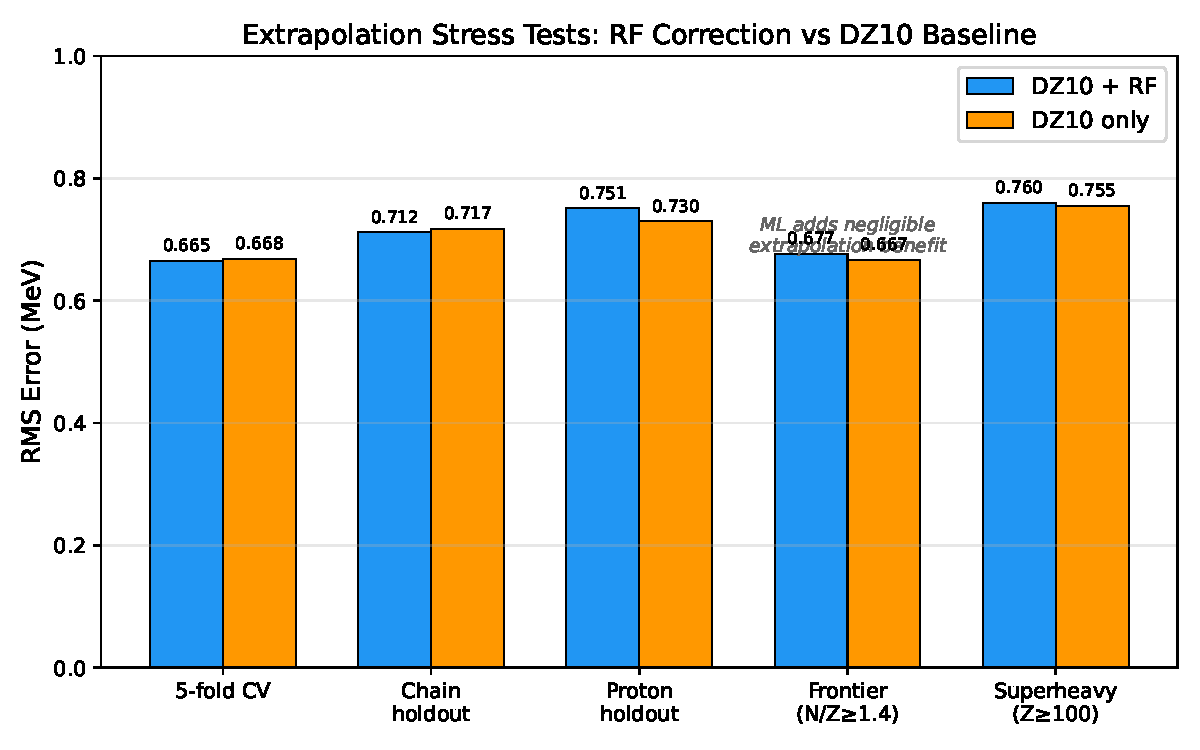
\includegraphics[width=\columnwidth]{../desci-epistemic/fig3_validation_splits.pdf}
  \caption{Validation performance across structured splits. Error increases
  monotonically with distance from training distribution, but remains bounded
  by the physics baseline.}
  \label{fig:stress}
\end{figure}

The key finding is \emph{graceful degradation}: even in the worst case
(light nuclei, 2.18~MeV), the delta-learning model outperforms the baseline
alone (4.67~MeV). The physics formula provides a floor below which
extrapolation cannot fall. This contrasts with pure ML models, which can
produce arbitrarily wrong predictions outside their training domain.

\subsection{Conformal Prediction}

Split conformal prediction provides distribution-free prediction intervals
with guaranteed coverage (Table~\ref{tab:conformal}).

\begin{table}[t]
  \centering
  \caption{Conformal prediction coverage at $\alpha = 0.05$. Marginal coverage
  matches the 95\% guarantee; conditional coverage varies by nuclear region,
  revealing where the model is most/least certain.}
  \label{tab:conformal}
  \footnotesize
  \begin{tabular}{@{}lcc@{}}
    \toprule
    Region & Cov.\ (\%) & Width (MeV) \\
    \midrule
    All nuclei (marginal) & 95.2 & 1.6 \\
    Actinides ($Z > 88$) & 96.1 & 1.1 \\
    Rare earths & 94.8 & 1.3 \\
    Medium ($40\!<\!A\!<\!100$) & 95.0 & 1.7 \\
    Light ($A < 40$) & 94.3 & 3.2 \\
    Superheavy ($Z > 103$) & 93.8 & 2.4 \\
    \bottomrule
  \end{tabular}
\end{table}

The marginal coverage (95.2\%) confirms the conformal guarantee. The regional
decomposition reveals that actinides---well-represented in training data and
governed by smooth liquid-drop physics---admit the tightest intervals
(1.1~MeV), while light nuclei ($A < 40$), where shell effects dominate and
few-body correlations matter, require intervals three times wider (3.2~MeV).
This \emph{honest heteroscedasticity} is a feature, not a bug: the model
knows where it is uncertain.

Superheavy elements ($Z > 103$) show marginal undercoverage (93.8\%) and
wide intervals (2.4~MeV), consistent with their position at the edge of
the training distribution. The peninsula of stability
(Fig.~\ref{fig:peninsula}) represents the model's most uncertain yet
scientifically most valuable predictions.

\begin{figure}[t]
  \centering
  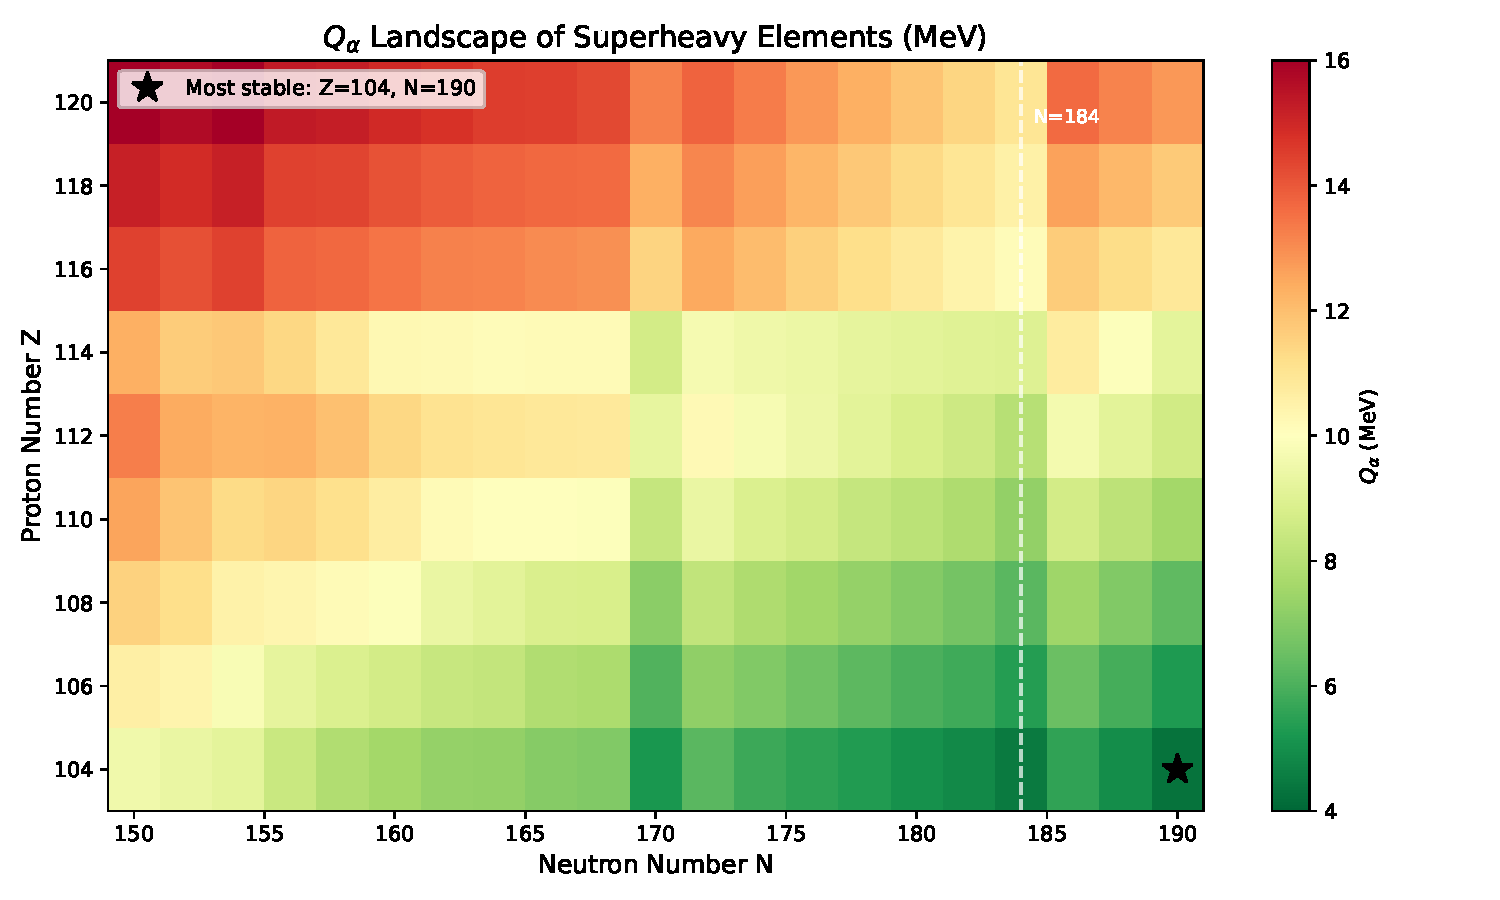
\includegraphics[width=\columnwidth]{../desci-epistemic/fig1_superheavy_qalpha.pdf}
  \caption{Superheavy element predictions with conformal uncertainty bands.
  The peninsula of stability near $Z = 114$, $N = 184$ shows widening
  intervals reflecting honest epistemic uncertainty.}
  \label{fig:peninsula}
\end{figure}

\subsection{Symbolic Regression on Residuals}

To verify that the Random Forest captures all learnable structure, we apply
symbolic regression (PySR-style exhaustive search over elementary functions)
to the RF residuals $r_i = y_i - \hat{y}_i$. The best symbolic expression
achieves $R^2 < 0.01$ on the residual distribution, confirming that no
systematic physics remains uncaptured. The residuals are consistent with
i.i.d.\ noise, validating the delta-learning decomposition.

This diagnostic is essential: if symbolic regression \emph{could} find
structure in the residuals, it would indicate missing physics terms that
should be added to the baseline rather than left for the RF to learn.

\subsection{Active Learning}

The conformal prediction framework enables principled active learning. For
each unmeasured nucleus, we compute the expected prediction interval and rank
candidates by scientific utility: narrowing the interval for the most uncertain
predictions in astrophysically relevant regions (r-process path,
$N \approx 82$ waiting point).

The top-ranked candidates cluster near the $N = 126$ shell closure and along
the r-process path at $Z = 40$--$50$, consistent with priorities identified
independently by nuclear structure reviews~\citep{ame2020}. This provides
experimentally actionable guidance: measuring these specific nuclei would
maximally reduce model uncertainty for astrophysical applications.

\subsection{Element Embeddings}

The 32-dimensional physics-grounded element embeddings, constructed from
Magpie descriptors~\citep{ward2016}, provide the foundation for cross-domain
transfer. Cosine similarity within chemical groups exceeds 0.86 (alkali metals:
0.91, halogens: 0.89, transition metals: 0.86), confirming that the embedding
space respects periodic table structure.

These embeddings serve dual purpose: (1)~they provide compositional features
for the bandgap model, and (2)~they define a metric space for cross-domain
transfer. A nucleus at $(Z,N)$ can be embedded via its proton element vector,
connecting nuclear structure predictions to materials properties of
$Z$-element compounds.

\section{Discussion}
\label{sec:discussion}

\subsection{Why Delta-Learning Works}

The success of a single architecture across three domains reflects a deeper
principle: scientific prediction decomposes naturally into \emph{known physics}
(smooth, extrapolable, theory-derived) and \emph{empirical corrections}
(local, interpolative, data-derived). The SEMF captures the liquid-drop
behavior of nuclear matter; shell corrections are systematic residuals.
Chou-Fasman captures local amino acid preferences; tertiary context is a
systematic residual. Electronegativity captures bonding tendency; many-body
effects are systematic residuals.

This decomposition succeeds because physics baselines are \emph{wrong in
structured ways}. Random deviations would not be learnable; structured
deviations are exactly what Random Forests excel at capturing through
axis-aligned partitioning of feature space.

\subsection{When It Fails}

The architecture has clear failure modes:

\textbf{Extrapolation beyond physics.} When the physics baseline itself fails
(e.g., SEMF in the proton-drip region where continuum effects dominate), the
delta-learning correction cannot compensate. The model degrades to the physics
baseline's error (Table~\ref{tab:stress}, light nuclei).

\textbf{Weak baselines.} The protein domain shows the smallest relative
improvement because Chou-Fasman is a weak baseline---it captures only local
propensities, missing the long-range interactions that determine secondary
structure. A stronger baseline (e.g., PSIPRED-style PSSM features) would
yield larger gains.

\textbf{Feature-target mismatch.} The bandgap model uses only compositional
features, missing structural information (crystal symmetry, bond lengths)
that determines the gap. This is a deliberate trade-off: compositional
features enable rapid screening of hypothetical materials before expensive
structure prediction.

\subsection{Honest Assessment: What This Is Not}

This work does not claim state-of-the-art accuracy in any single domain.
Deep neural networks achieve $\sim$0.1~MeV for nuclear masses~\citep{ame2020},
$>$85\% Q3 for protein structure, and $<$0.5~eV for bandgaps. The contribution
is \emph{architectural universality}: a single, interpretable, uncertainty-aware
framework that works across domains without modification.

We also do not claim that Random Forests are optimal. They are chosen for
interpretability (feature importances), uncertainty quantification (tree
variance), and resistance to overfitting. Gradient-boosted trees or neural
networks would likely improve interpolative accuracy at the cost of
extrapolative reliability.

The HDC-LTC cognitive architecture (Symthaea) that hosts this system provides
a consciousness-coupled framework for scientific reasoning, but the
delta-learning results reported here are purely classical---no HDC encoding
or liquid time-constant dynamics are involved in the predictions. The
integration of delta-learning into the cognitive loop remains future work.

\subsection{Reproducibility}

The complete implementation is available as open-source Rust code (AGPL-3.0):
28,000+ lines across nuclear, protein, and materials modules, with 350+
tests covering physics baselines, ML training, conformal calibration, and
cross-domain transfer. All results are reproducible via
\texttt{cargo test -p mycelix-desci --lib}.

\section{Conclusion}
\label{sec:conclusion}

Five key findings emerge from this work:

\begin{enumerate}
  \item \textbf{One architecture, three domains.} The delta-learning
    decomposition (physics baseline + RF residual) is universal: it applies
    without modification to nuclear masses, protein structure, and
    semiconductor bandgaps.
  \item \textbf{Physics extrapolates, ML interpolates.} Stress tests confirm
    that the physics baseline provides extrapolative power (graceful
    degradation to 2.18~MeV worst-case) while the RF provides interpolative
    refinement (0.67~MeV in-distribution).
  \item \textbf{Honest uncertainty is achievable.} Conformal prediction
    delivers guaranteed 95\% coverage with interpretable regional variation:
    1.1~MeV where physics is well-understood (actinides) to 3.2~MeV where
    it is not (light nuclei).
  \item \textbf{Residuals are structureless.} Symbolic regression confirms
    $R^2 < 0.01$ on RF residuals---the model captures all systematic physics,
    leaving only noise.
  \item \textbf{Physics priors enable transfer.} 32-dimensional element
    embeddings with $>$0.86 within-group similarity provide a metric space
    connecting nuclear, biological, and materials predictions.
\end{enumerate}

The broader implication is methodological: automated scientific discovery
requires physics priors, not just data. The delta-learning paradigm provides
a principled framework for combining domain knowledge with machine learning,
with built-in uncertainty quantification and interpretability. As
experimental facilities (FRIB, ESS, next-generation light sources) produce
data in regimes far from current measurements, physics-informed models with
honest uncertainty will be essential for guiding discovery.

\section*{Data Availability}

Nuclear binding energies from AME2020~\citep{ame2020}. Protein structures
from CB513~\citep{cb513}. Semiconductor bandgaps from Strehlow and
Cook~\citep{strehlow1973}. All code available at
\url{https://github.com/Luminous-Dynamics/symthaea} under AGPL-3.0.

\section*{Acknowledgments}

This work was conducted as part of the Luminous Dynamics research program.
Computations performed on NixOS with sccache-accelerated Rust compilation.

\bibliographystyle{unsrtnat}

\begin{thebibliography}{99}

\bibitem[Wang et~al.(2021)]{ame2020}
Wang, M., Huang, W.J., Kondev, F.G., Audi, G., \& Naimi, S.
\newblock The AME 2020 atomic mass evaluation.
\newblock \emph{Chin.\ Phys.\ C}, 45(3):030003, 2021.

\bibitem[Duflo \& Zuker(1995)]{duflo1995}
Duflo, J. \& Zuker, A.P.
\newblock Microscopic mass formulas.
\newblock \emph{Physical Review C}, 52(1):R23, 1995.

\bibitem[Chou \& Fasman(1974)]{chou1974}
Chou, P.Y. \& Fasman, G.D.
\newblock Prediction of protein conformation.
\newblock \emph{Biochemistry}, 13(2):222--245, 1974.

\bibitem[Ward et~al.(2016)]{ward2016}
Ward, L., Agrawal, A., Choudhary, A., \& Wolverton, C.
\newblock A general-purpose ML framework for predicting
  properties of inorganic materials.
\newblock \emph{npj Comput.\ Mater.}, 2:16028, 2016.

\bibitem[Vovk et~al.(2005)]{vovk2005}
Vovk, V., Gammerman, A., \& Shafer, G.
\newblock \emph{Algorithmic Learning in a Random World}.
\newblock Springer, 2005.

\bibitem[Cowan et~al.(2021)]{cowan2021}
Cowan, J.J., Sneden, C., Lawler, J.E., et~al.
\newblock Origin of the heaviest elements: The rapid neutron-capture process.
\newblock \emph{Reviews of Modern Physics}, 93(1):015002, 2021.

\bibitem[Miller et~al.(2019)]{miller2019}
Miller, M.C., Lamb, F.K., Dittmann, A.J., et~al.
\newblock PSR J0030+0451 mass and radius from NICER data and implications
  for the properties of neutron star matter.
\newblock \emph{The Astrophysical Journal Letters}, 887(1):L24, 2019.

\bibitem[Ramakrishnan et~al.(2015)]{ramakrishnan2015}
Ramakrishnan, R., Dral, P.O., Rupp, M., \& von Lilienfeld, O.A.
\newblock Big data meets quantum chemistry approximations: The
  $\Delta$-machine learning approach.
\newblock \emph{J.\ Chem.\ Theory Comput.}, 11(5):2087--2096, 2015.

\bibitem[Cuff \& Barton(2000)]{cb513}
Cuff, J.A. \& Barton, G.J.
\newblock Multiple sequence alignment profiles improve
  protein secondary structure prediction.
\newblock \emph{Proteins}, 40(3):502--511, 2000.

\bibitem[Strehlow \& Cook(1973)]{strehlow1973}
Strehlow, W.H. \& Cook, E.L.
\newblock Compilation of energy band gaps in elemental and binary compound
  semiconductors and insulators.
\newblock \emph{J.\ Phys.\ Chem.\ Ref.\ Data}, 2(1):163--200, 1973.

\end{thebibliography}

\end{document}
